\chapter{Macros}
TeXstudio permite crear macros. El perfil tiene implementadas tres para facilitar la escritura de comandos para las siguientes acciones:
\begin{enumerate}
	\item Añadir hiperenlace.
	\item Añadir \textit{snippets} de código.
\end{enumerate}

Además de crear la macro, se han incluido en la barra de herramientas superior y se les ha puesto iconos específicos. También se han puesto iconos específicos para los botones del entorno \textit{equations}, en la barra de herramientas lateral.

% TODO: \usepackage{graphicx} required
\begin{figure}[h]
	\centering
	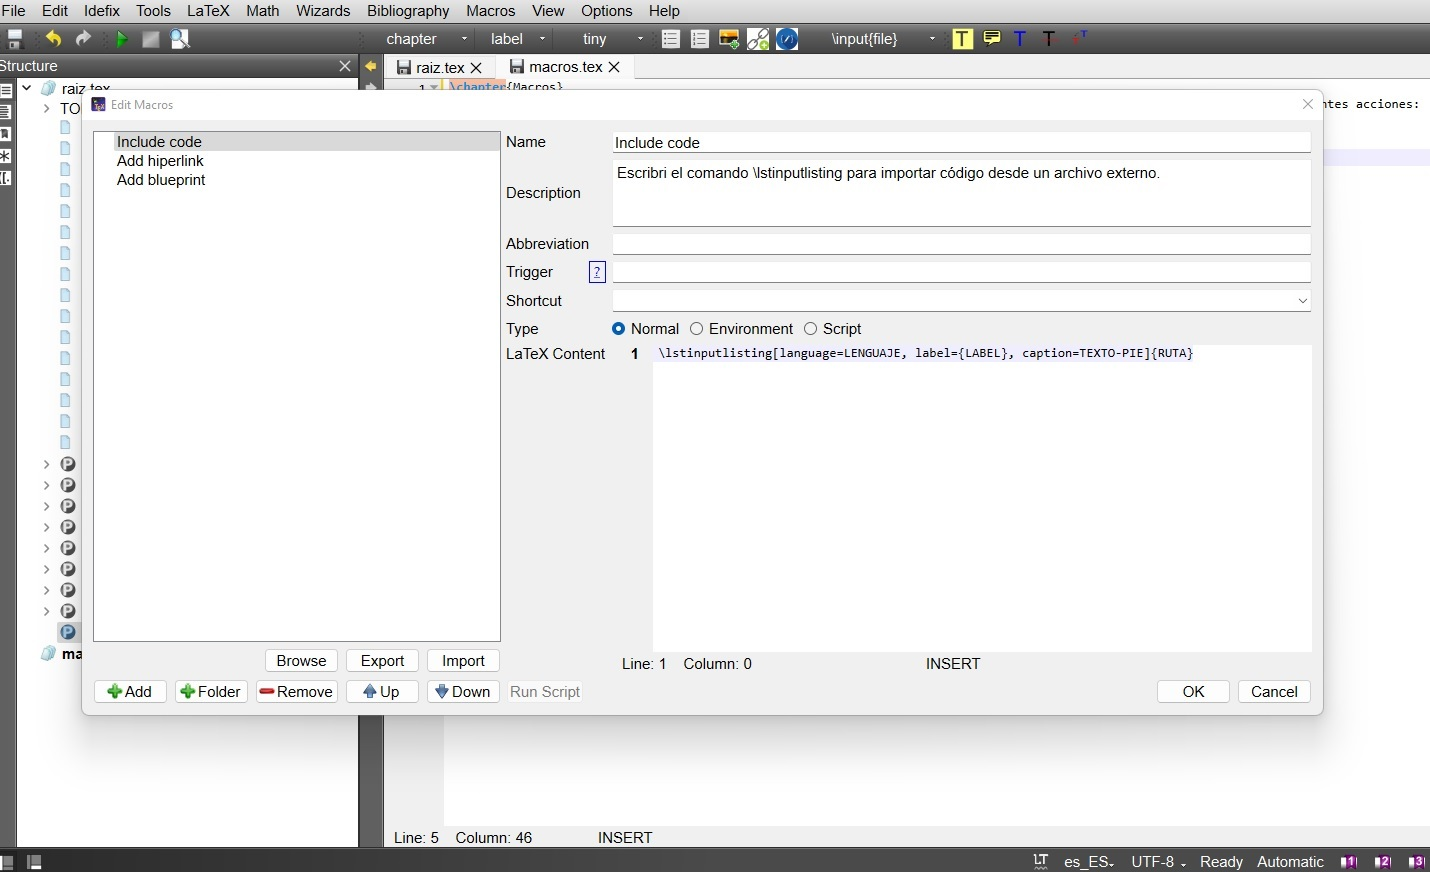
\includegraphics[width=1\linewidth, frame]{anexos/macros/imagenes/menu-macros}
	\caption[Menú Macros.]{Menú Macros. En este menú se pueden usar, crear y editar macros.}
	\label{fig:menu-macros}
\end{figure}

% TODO: \usepackage{graphicx} required
\begin{figure}[h]
	\centering
	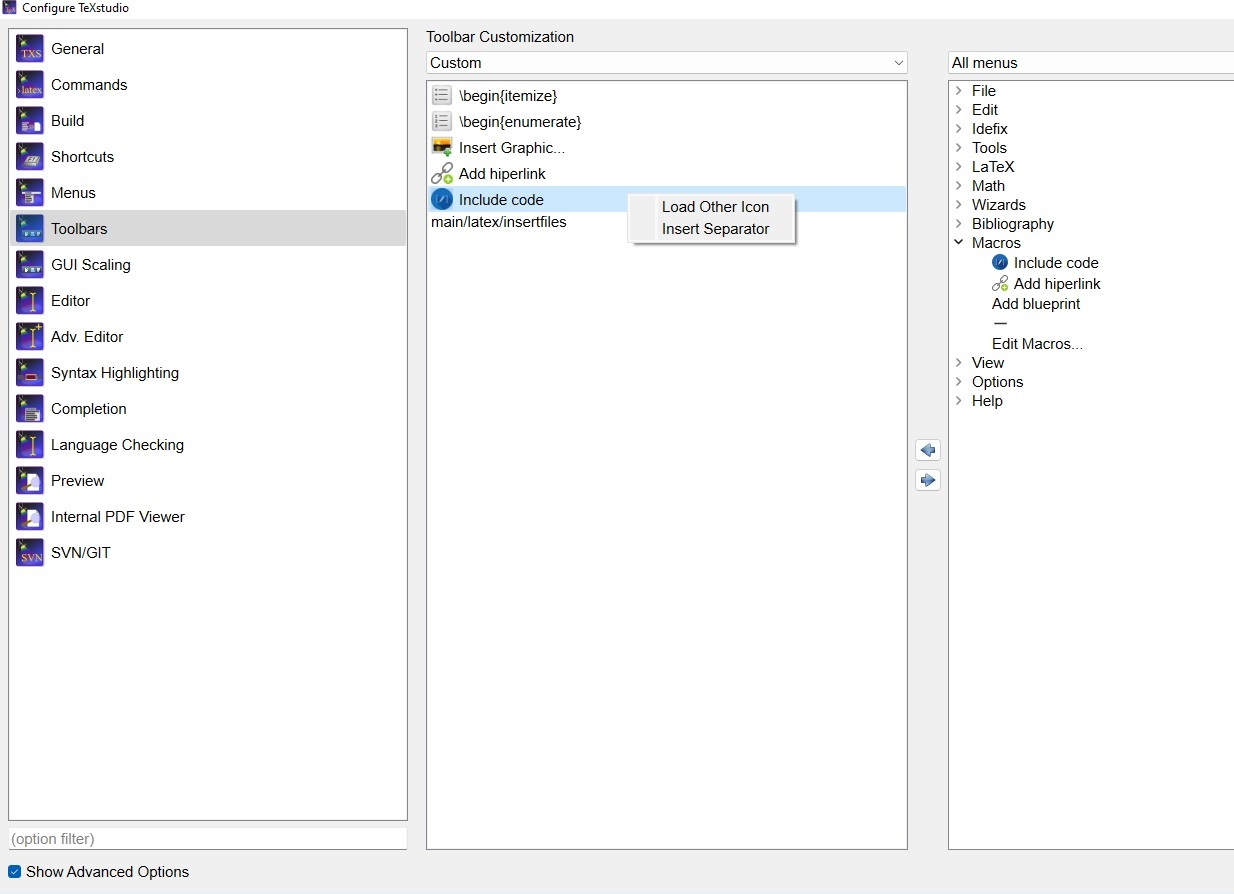
\includegraphics[width=1\linewidth, frame]{anexos/macros/imagenes/macros-boton-icono}
	\caption[Menú options/configuration/toolbars.]{Menú options/configuration/toolbars. En esta pantalla se pueden configurar las barras de herramientas, añadir botonoes e iconos.}
	\label{fig:macros-boton-icono}
\end{figure}

\begin{figure}[h]
	\centering
	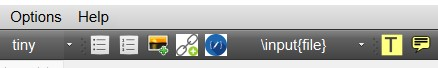
\includegraphics[scale=1, frame]{anexos/macros/imagenes/toolbar-sup}
	\caption[Barra de herramientas superior.]{Barra de herramientas superior. De izquierda a derecha los botones para las macros: tamaño de fuente, lista, enumeración, insertar imagen, insertar enlace, insertar código, insertar archivo; tras ellos botones para el paquete \textit{easyreview} para hacer comentarios de edición.}
	\label{fig:toolbar-sup}
\end{figure}

\begin{figure}[h]
	\centering
	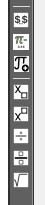
\includegraphics[scale=1, frame]{anexos/macros/imagenes/toolbar-lat}
	\caption[Barra de herramientas lateral.]{Barra de herramientas lateral. Los tres primeros botones, de arriba a abajo, son: entorno modo matemático, entorno ecuación numerada, entorno ecuación no numerada.}
	\label{fig:toolbar-lat}
\end{figure}
